\subsection{Summary of Curve Sketching}\label{subsec:SummaryCurveSketching}

The following is a guideline for sketching a curve $y=f(x)$ by hand. Each item may not be relevant to the function in question, but utilizing this guideline will provide all information needed to make a detailed sketch of the function.

\begin{formulabox}[Guideline for Curve Sketching]
\begin{enumerate}
	\item	Domain of the function
	\item	$x$- and $y$-Intercepts
	\item	Symmetry
	\item	Vertical and Horizontal Asymptotes
	\item	Intervals of Increase/Decrease, and Local Extrema
	\item	Concavity and Points of Inflection
	\item	Sketch the Graph
\end{enumerate}
\end{formulabox}

\begin{example}{Graph Sketching}{graphsketching}
Sketch the graph of $y=f(x)$ where $\ds{f(x)=\frac{2x^2}{x^2-1}}$
\end{example}

\begin{solution} 
\begin{enumerate}
\item  The domain is $\{x: x^2-1 \neq 0\}= \{x: x \neq \pm 1\}=(- \infty,-1) \cup (-1,1) \cup (1, \infty)$
\item  There is an $x$-intercept at $x=0$. The $y$ intercept is $y=0$.
\item  $f(-x)=f(x)$, so $f$ is an even function (symmetric about $y$-axis)
\item  $\ds{ \lim_{x \to \pm \infty} \frac{2x^2}{x^2-1} =\lim_{x \to \pm \infty} \frac{2}{1-1/x^2} = 2 }$, so $y=2$ is a horizontal asymptote.

Now the denominator is 0 at $x =\pm1$, so we compute:
\[\lim_{x \to 1^+} \frac{2x^2}{x^2-1} = + \infty, \;   \lim_{x \to 1^-} \frac{2x^2}{x^2-1} = - \infty, \;
\lim_{x \to -1^+} \frac{2x^2}{x^2-1} = - \infty, \;   \lim_{x \to -1^-} \frac{2x^2}{x^2-1} = + \infty.  \]
So the lines $x=1$ and $x=-1$ are vertical asymptotes. 

\item  For critical values we take the derivative:
$$f'(x) = \frac{4x(x^2-1)-2x^2 \cdot 2x}{(x^2-1)^2} = \frac{-4x}{(x^2-1)^2}.$$
Note that $f'(x)=0$ when $x=0$ (the top is zero).
Also, $f'(x)=DNE$ when $x=\pm 1$ (the bottom is zero).
As $x=\pm 1$ is \ifont{not} in the domain of $f(x)$, the only critical number is $x=0$ (recall that to be a critical number we need it to be in the domain of the original function).

Drawing a number line and including \ifont{all} of the split points of $f'(x)$ we have:
$$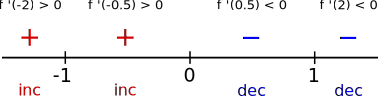
\includegraphics[width=3.5in]{images/graphex1}$$
Thus $f$ is increasing on $(-\infty, -1)\cup(-1,0)$ and decreasing on $(0,1)\cup(1, \infty)$.

By the first derivative test, $x=0$ is a local max.

\item  For possible inflection points we take the second derivative:
$$f''(x)= \frac{12x^2+4}{(x^2-1)^3}$$
The top is never zero.
Also, the bottom is only zero when $x=\pm 1$ (neither of which are in the domain of $f(x)$).
Thus, there are no possible inflection points to consider.

Drawing a number line and including \ifont{all} of the split points of $f''(x)$ we have:
$$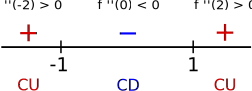
\includegraphics[width=2.25in]{images/graphex2}$$
Hence $f$ is concave up on $(- \infty,-1)\cup(1, \infty)$, concave down on $(-1,1)$.

\item  We put this information together and sketch the graph.

We combine some of this information on a single number line to see what \ifont{shape} the graph has on certain intervals:
$$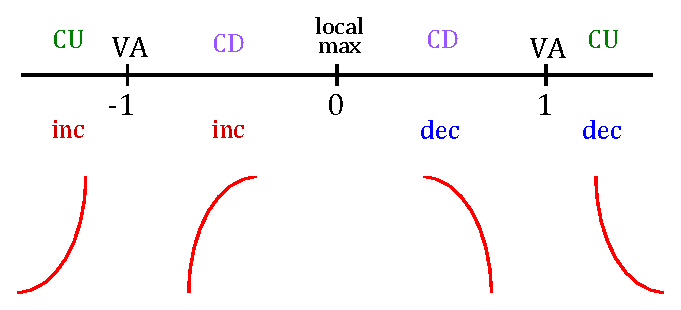
\includegraphics[width=3.0in]{images/graphex3}$$
Note that there is a horizontal asymptote at $y=2$ and that the curve has $x$-int of $x=0$ and $y$-int of $y=0$.
Therefore, a sketch of $f(x)$ is as follows:
$$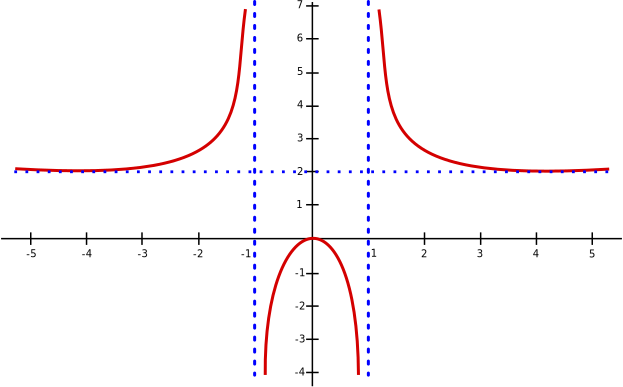
\includegraphics[width=3.5in]{images/graphex4}$$
\end{enumerate}
\end{solution}